\section{Wireframe}\label{s:wireframe}
La realizzazione dei wireframe è stata fatta mediante il software \textit{Balsamiq}; la loro realizzazione ha attraversato diverse iterazioni. Nelle seguenti sezioni presenteremo i vari wireframe e i widget che li compongono spiegando quali sono stati i nostri ragionamenti e le nostre iterazioni per raggiungere la versione finale.\\

\subsubsection{Header e footer}\label{ss:header-e-footer}
Ogni schermata possiede un header nella parte alta dello schermo e un footer nella parte bassa. I footer sono tutti uguali uguali, gli header sono simili in quanto presentano tutti un selettore di data, l'unico che differisce è quello della schermata ``Analisi di periodi'' che ne presenta due in quanto in quella schermata deve essere possibile, per il giornalista, inseire due range di date.

\begin{figure}[H]
    \centering
    
\includegraphics[width=1\columnwidth]{wireframes/header-una-data}
    \caption{Header di ``Panoramica'', ``Confronto fra regioni'' e ``Distribuzione su dati anagrafici''.}
    \label{fig:header-una-data}
\end{figure}

\begin{figure}[H]
    \centering
    
\includegraphics[width=1\columnwidth]{wireframes/header-due-date}
    \caption{Header di ``Analisi di periodi''.}
    \label{fig:header-due-date}
\end{figure}

Gli headers sono composti, partendo da destra:
\begin{itemize}
    \item logo della protezione civile;
    \item titolo della dashboard;
    \item selettore di date (due in \ref{fig:header-due-date}) composto da:
        \begin{itemize}
            \item freccia a sinistra, un bottone per passare al giorno precedente a quello indicato;
            \item bottone per aprire il widget per selezionare la data (\ref{} e \ref{});
            \item freccia a destra, simile alla freccia a sinistra ma con comportamento opposoto, cambia la data al giorno successivo rispetto a quello indicato (se la da ta è valida).
        \end{itemize}
\end{itemize}

I widget per selezionare la data, apribili tramite il bottone tra le due frecce, sono di due tipi. Uno se la pagina richiede  di inserire un singolo giorno e l'altro se la pagina richiede di inserire  un range di date.\\

\begin{figure}[H]
    \centering
    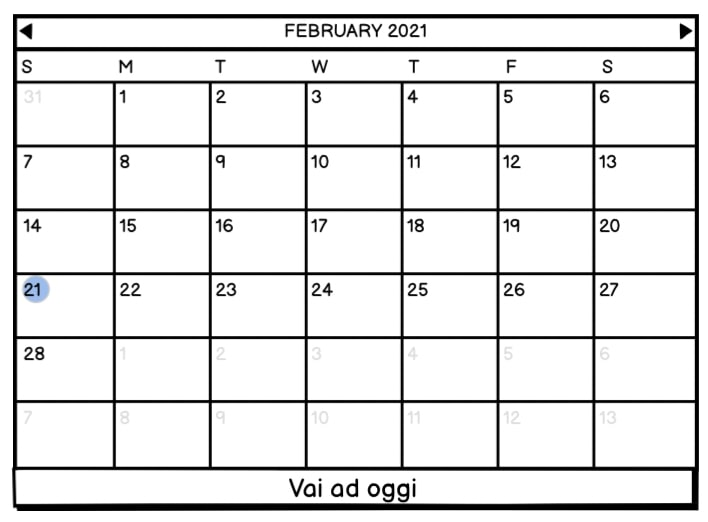
\includegraphics[width=0.3\columnwidth]{wireframes/header-data-singola}
    \caption{Widget per selezionare una data singola.}
    \label{fig:header-data-singola}
\end{figure}

\begin{figure}[H]
    \centering
    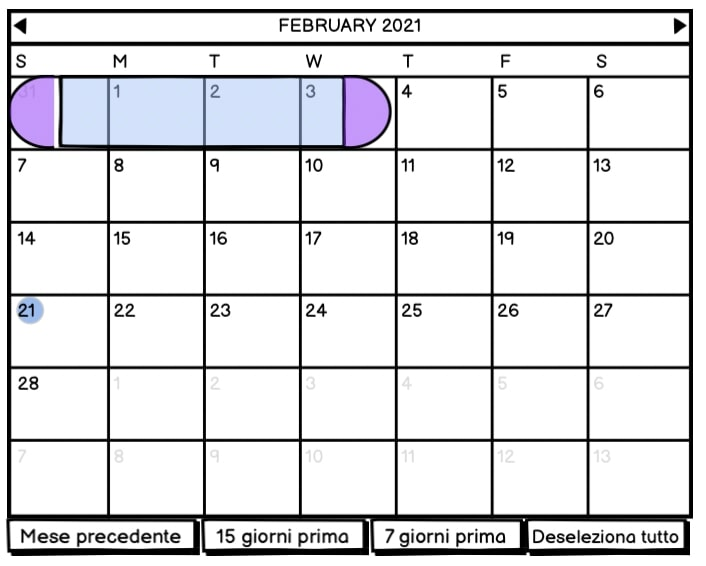
\includegraphics[width=0.3\columnwidth]{wireframes/header-data-range}
    \caption{Widget per selezionare un range di date.}
    \label{fig:header-data-range}
\end{figure}

\begin{figure}[H]
    \centering
    
\includegraphics[width=1\columnwidth]{wireframes/header-data-aperta}
    \caption{Header con data aperta.}
    \label{fig:header-data-aperta}
\end{figure}

Nel widget per selezionare una data singola (\ref{fig:header-data-singola}) vi è un bottone per tornare rapidamente alla data odierna.\\
Nel widget per selezionare un range di date (\ref{fig:header-data-range}) vi sono diversi bottoni che permettono di velocizzare alcune operazioni come: andare al mese precednete, ai quindici giorni precedenti, ai sette giorni precedenti e per deselezionare il range.\\
In \ref{fig:header-data-aperta} vi è una dimostrazione di come il widget appare rispetto all'header.

\begin{figure}[H]
    \centering
    
\includegraphics[width=1\columnwidth]{wireframes/footer}
    \caption{Footer comune a tutte le schermate}
    \label{fig:footer}
\end{figure}

Nel footer (\ref{fig:footer}) vi sono alcune informarzioni e link per le pagine istituzionali e le fonti dai quali i dati sono stati recuperati; da destra ci sono:
\begin{itemize}
    \item logo della Repubblica Italiana;
    \item logo e nome della Protezione Civile;
    \item link alle fonti e data dell'ultimo aggiornamento;
    \item link ai siti istituzionali.
\end{itemize}

\subsubsection{Panoramica}\label{ss:panoramica}
%TODO: Inserire figura


\subsubsection{Confronto fra regioni}\label{ss:confronto-fra-regioni}

\subsubsection{Analisi di periodi}\label{ss:analisi-di-periodi}

\subsubsection{Distrubuzione su dati anagrafici}\label{ss:distribuzione-su-dati-anagrafici}
